
\documentclass{article}
\usepackage[utf8]{inputenc}
\usepackage[margin=1in,left=1.5in,includefoot]{geometry}
\usepackage{booktabs}
\usepackage{graphicx}
\usepackage{amsmath}
\usepackage[spanish]{babel}

% Header & Footer Stuff

\usepackage{fancyhdr}
\pagestyle{fancy}
\lhead{Modelos Avanzados de Aprendizaxe Automático II}
\rhead{614G030302425}
% \fancyfoot{}
% \lfoot{Pablo Chantada Saborido \& José Romero Conde}
% \fancyfoot[R]{}

% The Main Document
\begin{document}
\begin{center}
    \LARGE\bfseries PRÁCTICA III \\
    \large \emph{Aprendizaxe por reforzo} \\
    \small Pablo Chantada Saborido \& José Romero Conde
    \line(1,0){430}
\end{center}

\vspace{200}
\begin{figure}[h]
    \centering
    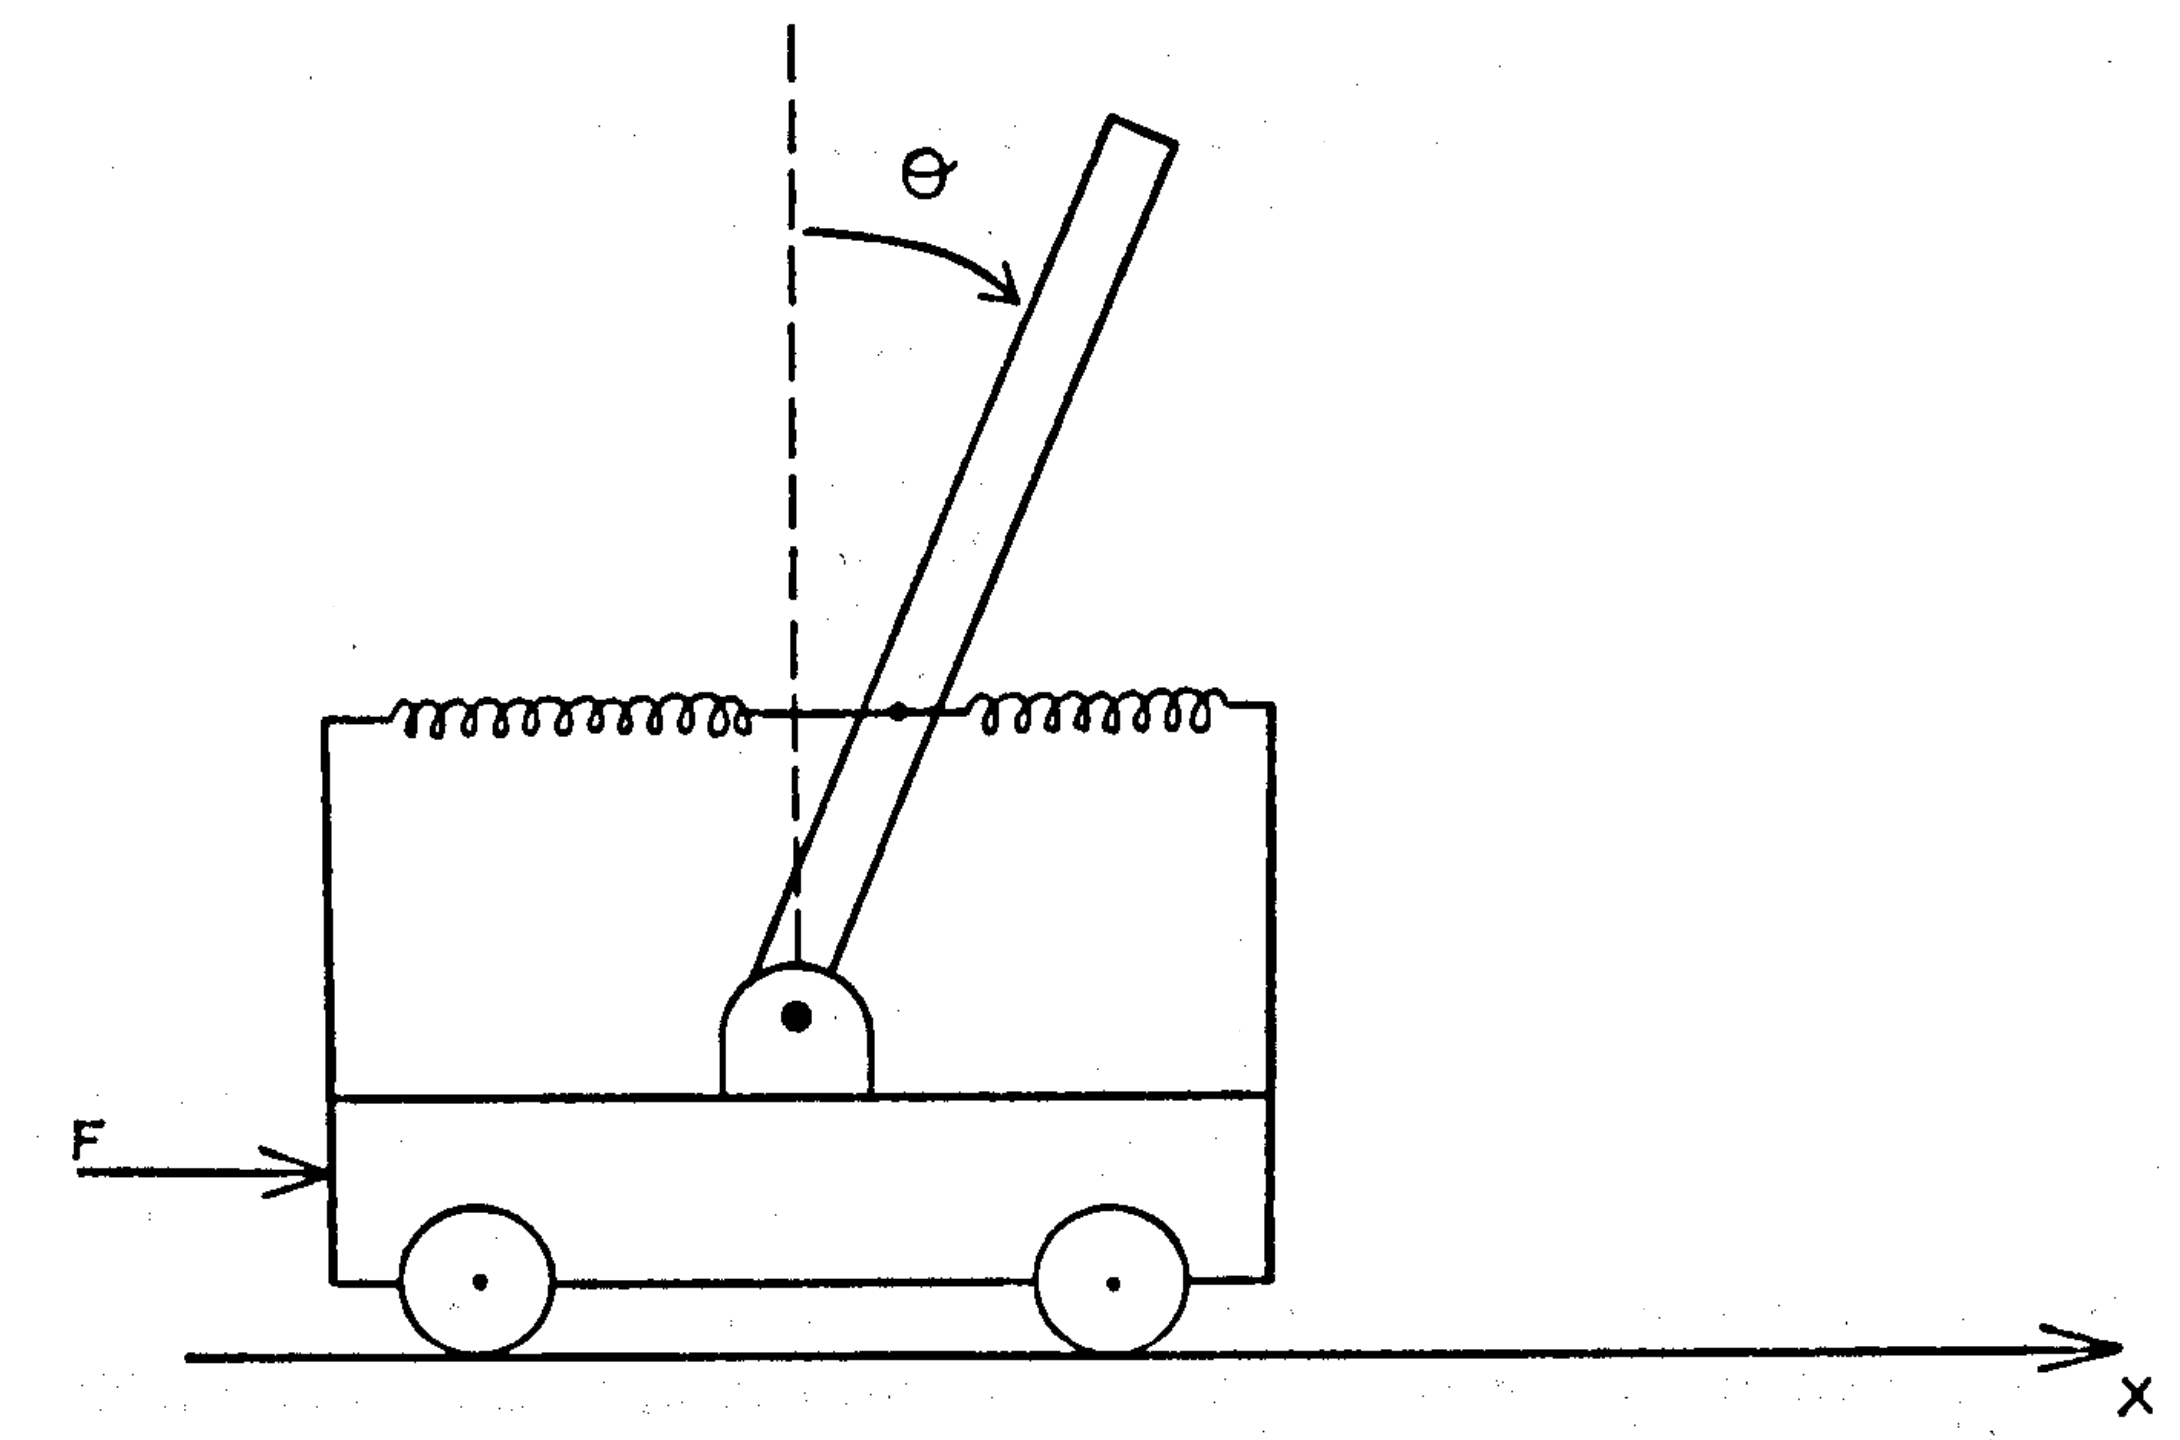
\includegraphics[width=1\linewidth]{portada.png}
    
    \label{fig:enter-label}
\end{figure}

\thispagestyle{empty}
\newpage

\section{Introdución e aspectos xerais}

Sobre a programación, comentar:

\begin{figure}[h]
    \centering
    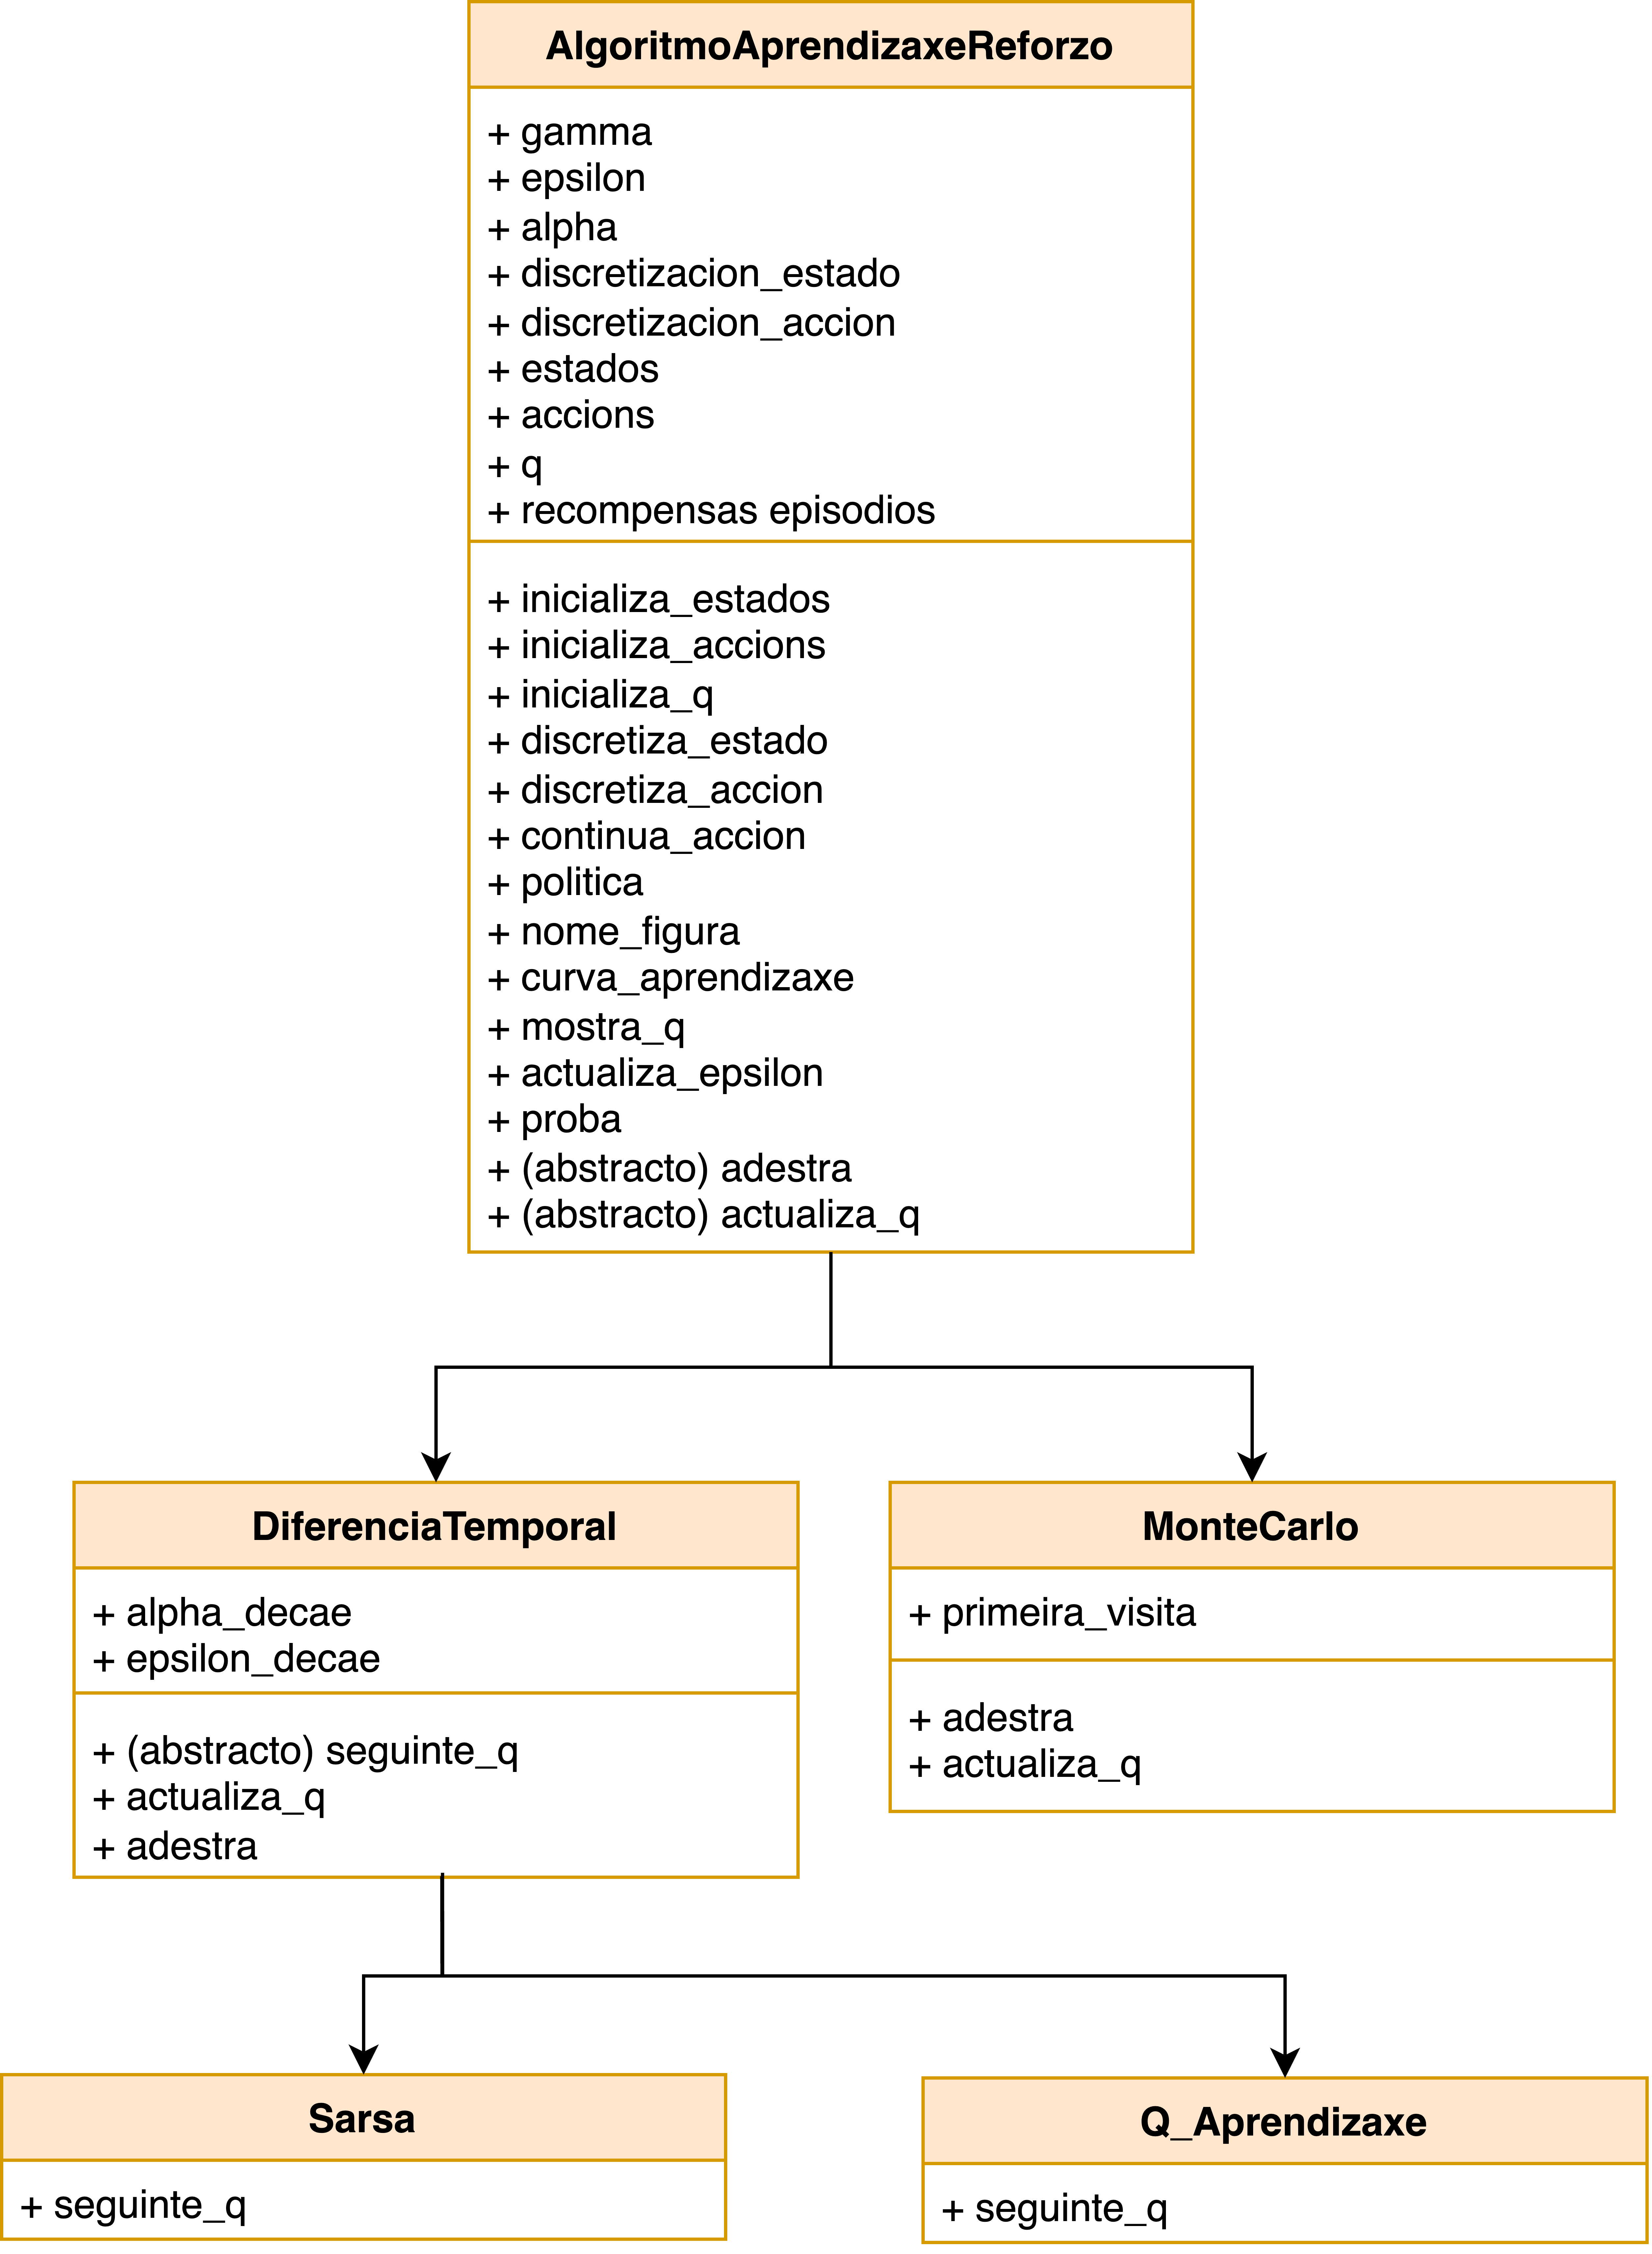
\includegraphics[width=0.7\linewidth]{herencia.drawio.png}
    
    \label{fig:enter-label}
\end{figure}

\section{Hiperparámetros}
¿Qué hiperparámetros has utilizado? ¿Cómo has seleccionado estos
hiperparámetros? ¿Por qué son más adecuados que otros valores?

\section{Mellor política determinista}
\section{Mellor algoritmo de control}
\section{Perturbacións}
\section{Conclusións}

\newpage

For the
control problem (finding an optimal policy), DP, TD, and Monte Carlo meth-
ods all use some variation of generalized policy iteration (GPI). The differences
in the methods are primarily differences in their approaches to the prediction
problem.


Although Q-
learning actually learns the values of the optimal policy, its on-line performance
is worse than that of Sarsa, which learns the roundabout policy. Of course, if
ε were gradually reduced, then both methods would asymptotically converge
to the optimal policy.



\newpage

\bibliographystyle{plain}  % or another style like "ieeetr", "acm", "alpha", etc.
\bibliography{articulos_mencionados}  % 'references' is the name of your .bib file (without the extension)



\end{document}

